\section{Introduction}
\label{sec:intro}


% % Edge Infrastructures are the next platform
% With the emergence of Network Function Virtualization (NFV)
% technologies as well as Internet of Things (IoT) and augmented/virtual
% reality (AR/VR) applications, Cloud and Network communities are
% advocating for going towards massively distributed small sized
% infrastructures that are deployed at the edge of the network.
% %
% Referred to as the Edge Computing paradigm, this model aims at
% delivering Cloud Computing capabilities closer to end-users, their
% related devices, and applications.
% %

While several academic studies have been highlighting the advantages
of the Edge Computing paradigm in various
domains~\cite{bonomi2012fog,satyanarayanan2017emergence,shi2016edge,yi2015fog,zhang2015cloud},
%%
progress on how operating and using infrastructures that serve it are marginal.
Current solutions~\cite{akamai:cloudlets}~\cite{amazon:lambda-edge} are rather close to the
initial fog proposal that allows to run domain-specific applications
on  NFV-enabled infrastructures (at the edge) and
centralized clouds~\cite{bonomi2012fog}.  In other words, %current Edge Infrastructure-as-a-Service (IaaS)
these solutions do not allow to run stateful
workloads in isolated environments, \eg{ containers or virtual	machines (VMs)}.
%
This is surprising as DevOps expect to find most features that make the sucess of
current Cloud Computing solutions.

% Our community should tackle the challenge of delivering a general
% resource management system to operate and use Edge Computing
% infrastructure. Something that will first, let an operator aggregates,
% supervises and exposes the massively distributed resources of the
% infrastructure and second, let a developer implements new kinds of
% services on top of that infrastructure that may be deployed and
% managed on demand.

%% Thus, the development of a general resource management system to
%% operate and use Edge Computing infrastructures is still an open
%% question.

%% %%  We need a resource management system that enables administrators to
%% %% operate and end-users to use edge resources.
%% %% a resource management system that will enable, on the one hand,
%% %% an operator to aggregate, supervise and expose such massively
%% %% distributed resources and, on the other hand, a developer to implement
%% %% new kinds of services that may be deployed and managed on demand is
%% %% still an open question.

%% %%  Delivierng en Edge IaaS system is complex
%% Domain specific solutions~\cite{bonomi2012fog} allow IoT applications
%% to run on infrastructures composed of NFV-enabled hardware (at the
%% edge) and existing centralized clouds. However, these solutions do not
%% allow to run workloads in isolated environments such as containers or
%% virtual machines (VMs).
%% %
%% This is rather critical as developers/end-users expect to find
%% most features that makes the success of current Cloud Computing solutions.

%% Requirements:
%%
%% 1. il y a des fonctionnalités spécifiques au edge
%%
%% 2. on a étudié différentes stratégies de design d'une IaaS manager
%%    qui implementerait nos requieremtn avec comme *contraintes de
%%    réutilier au plus les VIM*.

%% Les implem essaye de réutiliser les VIM pour minimiser l'effort de
%% dvlp. Elle font ceci par aggrega des API, mais le problème est
%% qu'elles se limite à être des gestionnaires de resources (cf k8s
%% discussion avec Adrien) alors que un VRAIE IaaS manager doit
%% considérer plus de chose (donner un exemple de req).

%On this basis,
%
The ETSI Mobile Edge Computing Industry Specification Group
defined in 2016 an architecture to orchestrate distinct
independent Cloud systems, \aka Virtual
Infrastructure Managers (VIM) ~\cite{7574435}.
%
The idea consists in federating VIMs of the several Data Centers (DCs) that
compose the Edge infrastructure.  By reusing VIMs, ETSI targets an Edge
Computing resource management that behaves in a same fashion as Cloud
Computing, while mitigating development requirements.
%
Although there is no implementation available, the idea of federating
VIMs seems promising as several projects have been built on similar
concepts. ONAP~\cite{onap}, an industry-driven solution,
enables the orchestration and automation of virtual network functions
across distinct VIMs. From the academic side, FogBow~\cite{brasileiro2016fogbow} aims to support federations
of Infrastructure-as-a-Service (IaaS) providers. More recently, NIST
initiated a collaborative effort with IEEE to advance Federated
Cloud through the development of a conceptual architecture and a
vocabulary\endnote{\url{https://collaborate.nist.gov/twiki-cloud-computing/bin/view/CloudComputing/FederatedCloudPWGFC}
  (March 2018).}.

All these projects provide valuable contributions, unfortunately they have
been all designed by only considering the DevOps' perspective. They provide
abstractions to manage the life cycle of geo-distributed applications,
but do not address administrative requirements.
%
However, Edge Computing infrastructures differ from federated cloud systems
in various aspects~\cite{openstack:whitepaper}, for instance:
Edge sites are potentially unmanned and therefore must be administered remotely;
management systems should be designed to cope with intermittent network access to sites; distinct operators might be interested in interconnecting their infrastructures (like network peering).
%

To favor the advent of Edge Computing, our community should take part
of current discussions and actions in order to deliver a well-suited
resource management system. A system that will first, let an operator aggregate, supervise and expose the massively distributed resources of the infrastructure,
and second, let DevOps implement new kinds of services on top of that infrastructure that may be deployed and managed on-demand.

% Designing and implementing a complete software stack to enable
% administrators to operate, and developers to use, distinct edge sites
% like a global Cloud Computing infrastructure is a difficult challenge
% for our community. However it is a challenge we should tackle soon to
% favor the advent of the Edge Computing paradigm.

In this paper, we present reflections to initiate discussions through our community.

\begin{itemize}[noitemsep, topsep=0pt]
\item First, we introduce a classification of expected features from
  both administrators and DevOps. This classification is valuable to
  identify missing mechanisms in resource management systems.
 % Moreover, it should deliver significant insights on the
 % design and implementation of a resource management system for the
 % edge computing.
\item Second, based on the identified requirements, we discuss
  how an Edge resource management system
  should be designed. In particular, we study \emph{pros} and
  \emph{cons} of \emph{top-down} and \emph{bottom-up} approaches. The
  former consists in interacting with each site only through
  exposed VIM APIs, such as in federated approaches. The
  latter aims at revising internal mechanisms of VIMs to enable native
  collaborations.
  \end{itemize}

\begin{figure}[t]
  \centering
  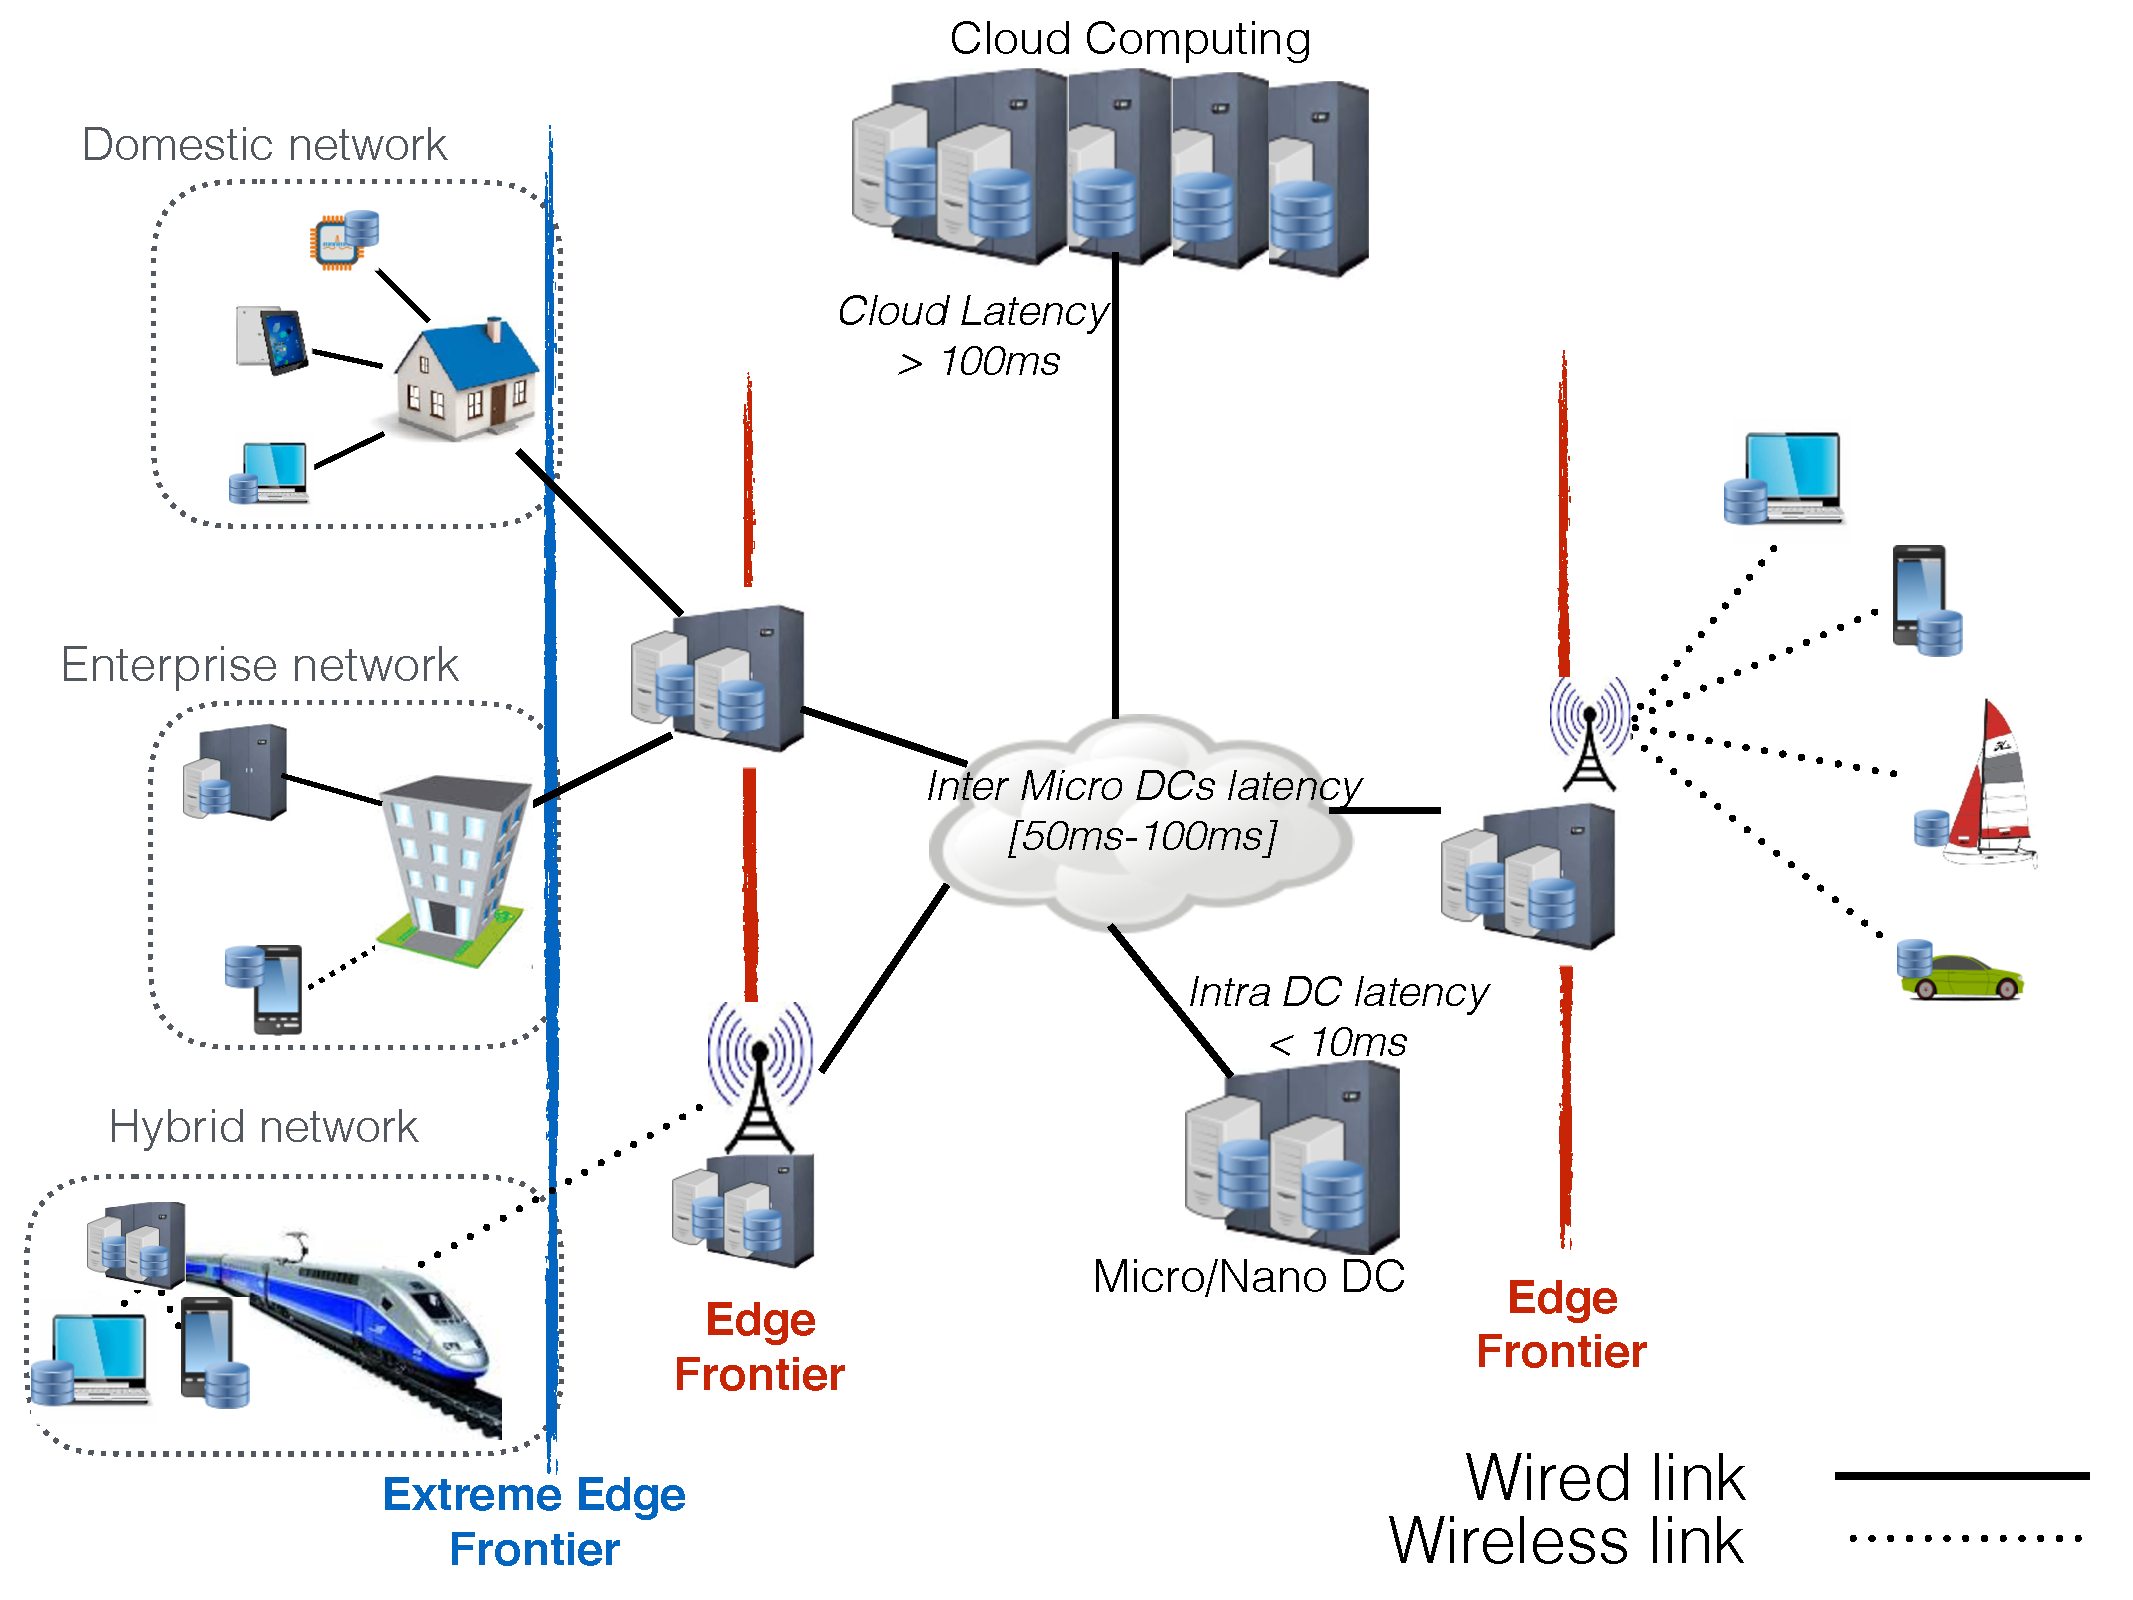
\includegraphics[width=\columnwidth]{./figures/figure_fog.pdf}
    \vspace*{-.5cm}
  \caption{Edge Computing Infrastructure~\cite{7923796}.}
    {\small The red dashed lines depict a split-brain situation that isolates
    \emph{Site 1} from other sites.}
  \label{fig:fogedge-archi}
  \vspace*{-.3cm}
\end{figure}

Since there are as many Edge infrastructures as use-cases, we
highlight that the infrastructure considered in this
study is composed
%, from the hardware viewpoint,
 of several
geo-distributed micro DCs (up to thousands)
composed of up to one hundred servers (nearly two racks).
Figure~\ref{fig:fogedge-archi} depictes such an infrastructure.
The expected latency and bandwidth between elements may fluctuate, in particular because
networks can be wired or wireless. Moreover, disconnections
between sites may occur leading to network split brain
situations~\cite{4456903}.
Finally, it is possible to consider additional DCs at the Extreme Edge, within private institutions or public transports.
%
From the software viewpoint, to simplify the model and
without loss of generality, we mainly assume OpenStack ~\cite{openstack:www} as the default VIM.  After years of development, OpenStack is today the de facto open-source solution to operate, supervise and use
IaaS infrastructures.
%More recently it has increased its effort to address edge computing cases.
%The OpenStack community gathers more than 500
%organizations, including large groups, in particular key actors of
%edge infrastructures such as ATT, Verizon~\ldots.

The remainder of the paper is organized as
follows. Section~\ref{sec:requirements} presents the major features
expected by administrators and DevOps.
%highlighting in particular differences \wrt federated infrastructures.
Section~\ref{sec:system_design_considerations} studies use of OpenStack for the Edge,
highlighting the need for effective collaboration across the
entire Edge infrastructure. Section~\ref{sec:design_discussion}
discusses two approaches that can be followed to
design a resource management system for the Edge, and points out a way forward. Section~\ref{sec:conclusion} concludes the paper.


% In this paper, we provide a list of expected features for both administrators and admins.
% We investigate whether a stack such as OpenStack, the defacto open-source standard can fullfil these requirements
% We finally discusss two possibles ways for moving forward: top/down vs bottom/up.
